\documentclass[12pt]{article}

\usepackage[a4paper]{geometry} %page size
\usepackage{parskip} %no paragraph indentation
\usepackage{fancyhdr} %fancy stuff in page header
\pagestyle{fancy} 

\usepackage[utf8]{inputenc} %encoding
\usepackage[danish]{babel} %danish letters

\usepackage{graphicx} %import pictures
\graphicspath{ {images/} }
\usepackage{listings} %make lists

\usepackage{amsmath, amssymb, amsfonts, amsthm, mathtools} %doing math
\usepackage{algorithmicx, algpseudocode} %doing pseudocode

\title{
  Title\
  \large Subtitle
}
\author{Asger Andersen}
\date{\today}

\fancyhead{}
\lhead{Miniprojekt 1}
\rhead{Asger Andersen}

%End of preamble
%*******************************************************************************

\begin{document}

\section{Disposition}

Jeg vil gerne gennemgå opgave 3. Jeg vil forsøge at anlægge et perspektiv, hvor jeg fokuserer mere på de overordnede principper og bagvedliggende intutioner end konkrete udregninger.

\begin{itemize}
\item Præsentation og udledning af modellen
\item Ligevægte for modellen. Abstrakt såvel som konkrete. Fortolkning.
\item Stabilitet af ligevægtene (herunder funktionalmatricer og egenværdier). Fortolkning.
\item Ligevægte for en mere kompliceret model.
\end{itemize}

\section{Udregninger}

Vi vil gerne modellere en modellere en epidemis udvikling over tid med en SIR. Det vil sige, at vi opdeler populationen af $N$ individer i tre grupper, nemlig $M_t$ (antallet af modtagelige individer til tid $t$), $S_t$ (antallet af smittede individer til tid $t$) og $I_t$ (antallet af immune individer til tid $t$). 

Vi antager, at antallet af nye smittede individer til tid $t$ er propertionelt med både antallet af smittede og antallet af modtagelige til tid $t$. Vi antager også, at en fast andel $a$ af de smittede til tid $t$ bliver immune til tid $t+1$. Altså får vi
\begin{align}
S_{t+1} = (1-a)S_t + \frac{b}{N}S_tM_t, \qquad 0<a<1,\quad 0<b
\end{align}

Vi antager også, at en fast andel $c$ af de immune til tid $t$ bliver ikke-immune til tid $t+1$. Altså får vi
\begin{align}
I_{t+1} = (1-c)I_t + aS_t
\end{align}

Vi antager, at ingen af dem, der bliver ikke-immune i periode $t$ bliver syge i periode $t$. Altså bliver de alle sammen modtagelige. Altså får vi, at antallet af modtagelige i periode $t+1$ er antallet af modtagelige i periode $t$ minus den andel, der bliver smittede i periode $t$, plus den andel der bliver ikke-immune i periode $t$:
\begin{align}
M_{t+1} = M_t - \frac{b}{N}S_tM_t + cI_t
\end{align}

Vi kan udnytte, at 
\begin{align}
M_{t+1} + S_{t+1} + I_{t+1} = M_t + S_t + I_t = N
\end{align}
til at forsimple modellen ved at substituere $M_t = N - S_t - I_t$ ind i ligningen for $S_{t+1}$. Hermed får vi systemet
\begin{align}
S_{t+1} = (1-a)S_t + bS_t\left(1 - \frac{S_t + I_t}{N}\right)\\
I_{t+1} = (1-c)I_t + aS_t
\end{align}
Dette er et autonomt, ikke-linært system af differens-ligninger.

Lad mig nu udregne betingelserne for, om modellen har ligevægte skarpt større end 0.

Lad $0 < N, b$ og $0 < a,b < 1$. 

$(S^*,I^*)\in \mathbb{R}^2$ er en ligevægt for modellen, hvis og kun hvis
\begin{align}
S^* = (1-a)S^* + bS^*\left(1 - \frac{S^* + I^*}{N} \right)\\
I^* = (1-c)I^* + aS^*
\end{align}
Det er let at se, at uanset værdien af $a, b, c$ og $N$, så vil $(S^*,I^*)=(0,0)$ altid være en løsning af disse ligninger. Ved hjælp af kedsommelige regnerier kan vi desuden komme frem til, at hvis $(S^*,I^*)\neq(0,0)$, så er $(S^*,I^*)$ en løsning til ovenstående ligningssystem, hvis og kun hvis
\begin{align}
S^* = c\Gamma(N,a,b,c), \quad I^* = a\Gamma(N,a,b,c)
\end{align}
hvor vi har defineret
\begin{align}
\Gamma(N,a,b,c) =  \frac{N(b-a)}{b(a+c)}
\end{align}
Vi ser, at modellen har en ligevægt $(S^*, I^*)$, hvor $0<S^*, I^*$, hvis og kun hvis $b>a$. Det giver mening, at $b$ skal være skarpt større end $a$ for at vi kan få en ligevægt med et positivt antal smittede, da $b$ angiver smitteraten og $a$ angiver immuniseringsraten.

Det gælder om denne ligevægt, at 
\begin{align}
\frac{S^*}{I^*} = \frac{c}{a}
\end{align}
Det giver mening, da $a$ er andelen af smittede, der bliver immune hver periode, og $c$ er andelen af immune, der bliver ikke-immune hver periode.

Dette passer også med, at sætter vi $N=100000, a=0.3, b=1.8$ og $c=0.1$ og fremskriver værdierne af $(S_t, I_t)$ ud fra startvektoren $(S_0, I_0)=(1000,0)$, så får vi dette plot
\begin{center}
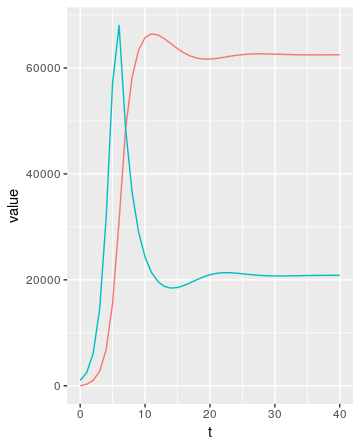
\includegraphics[scale=0.5]{q3p1.png}
\end{center}
hvor den blå graf er antallet af syge og den røde er antallet af immune. Her er $a>b$ og modellen ser ud til at have en ligevægt med $S^*$ omkring 21000 og $I^*$ omkring 62000. Laver vi samme plot med $b=0.2$, så får vi
\begin{center}
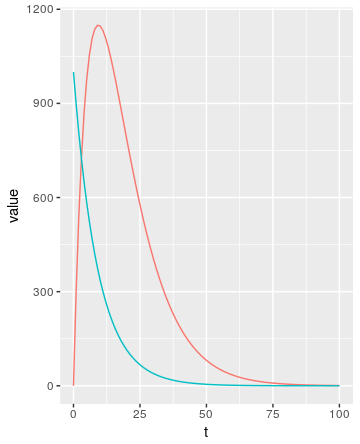
\includegraphics[scale=0.5]{q3p2.png}
\end{center}
Her er $b<a$ og modellen ser ud til at have ligevægten $(S^*, I^*)=(0,0)$. 

Lad os beregne alle ligevægte for $N=100000, a=0.3, b=1.8$ og $c=0.1$. Som sagt har vi altid ligevægten $(S^*, I^*)=(0,0)$. Bruger vi det generelle resultat fra linje (34-35), får vi desuden ligevægten $(S^*, I^*)=(20833.\overline{33},62500)$. Dette passer med, hvad vi så i plottet ovenfor.

Jeg vil nu finde ud af, om disse ligevægte er stabile. Jeg udregner funktionalmatricen for vores epidemimodel til
\begin{align}
\begin{bmatrix}
1 - a + b - b\frac{2S + I}{N} && - \frac{bS}{N} \\
\\
1-c && a 
\end{bmatrix}
\end{align}
Indsætter vi $N=100000, a=0.3, b=1.8, c=0.1, S=0$ og $I=0$ i funktionalmatricen, får vi matricen
\begin{align}
\begin{bmatrix}
2.5 && 0 \\
\\
0.9 && 0.3 
\end{bmatrix}
\end{align}
Den har egenværdierne $2.5$ og $0.3$, hvilket vil sige, at ligevægten $(0,0)$ ikke er lokalt stabilt, da $1\leq |2.5|$.

Indsætter vi $N=100000, a=0.3, b=1.8, c=0.1, S=20833.\overline{33}$ og $I=62500$ i funktionalmatricen, får vi matricen
\begin{align}
\begin{bmatrix}
0.625 && 0.375 \\
\\
0.9 && 0.3 
\end{bmatrix}
\end{align}
Den har egenværdierne $0.4625 + 0.5\overline{57}i$ og $0.4625 - 0.5\overline{57}i$, som begge har modulus $\sqrt{0.4625^2 + 0.5\overline{57}^2}=0.725<1$. Altså er ligevægten $(20833.\overline{33}, 62500)$ lokalt stabil.

\subsection{Delopgave e}

Lad $0 < N, b$ og $0 < a,b < 1$. 

$(S^*,I^*)\in \mathbb{R}^2$ er en ligevægt for den modificerede model, hvis og kun hvis
\begin{align}
S^* = (1-a)S^* + b(S^*)^2\left(1 - \frac{S^* + I^*}{N} \right)\\
I^* = (1-c)I^* + aS^*
\end{align}
Igen er det let at se, at uanset værdien af $a, b, c$ og $N$, så vil $(S^*,I^*)=(0,0)$ altid være en løsning af disse ligninger. 

For at bestemme andre løsninger til systemet, kan vi starte med at omskrive til det ækvivalente ligningssystem
\begin{align}
0 = -a + bS^*\left(1 - \frac{S^* + I^*}{N} \right)\\
I^* = \frac{c}{a}S^*
\end{align}
Indsætter vi udtrykket for $I^*$ fra den nederste ligning i den øverste, får vi
\begin{align}
0 = -a + bS^*\left(1 - \frac{S^* + \frac{c}{a}S^*}{N} \right)
\end{align}
Vi ser at dette er en andengradsligning og omskriver den ved hjælp af en masse regnerier til den konventionelle form
\begin{align}
0 = \left(\frac{bc}{aN} + \frac{b}{N} \right)(S^*)^2 + bS^* + a
\end{align}
Hermed får vi diskriminanten
\begin{align}
d = b\left(\frac{bN - 4(a+c)}{N}\right)
\end{align}
som er skarpt større end 0, hvis og kun hvis
\begin{align}
bN > 4(a+c)
\end{align}
Hvis dette er opfyldt, så får vi altså - udover nulløsningen - to løsninger givet ved
\begin{align}
S^* = \frac{b \pm \sqrt{d}}{2\left(\frac{bc}{aN} + \frac{b}{N} \right)}\\
I^* = \frac{c}{a}S^*
\end{align}
Disse er forskellige fra nulløsningen, hvis og kun hvis
\begin{align}
\sqrt{d} \notin \{-b,b\}
\end{align}
Hvis linje (42) og (45) er sande, så har modellen altså to ligevægte, der er forskellige fra $(0,0)$. 

\end{document}